\chapter{Aldagai anitzeko funtzioak}
\section{Aldagai anitzeko funtzioen jarraitutasuna}
\underline{10.2.ariketa} Aztertu funtzio honen jarraitutasuna jatorrian.
$$f(x,y) = \left\{ \begin{array}{cl}
		x\sin \dfrac{1}{y} +y \sin \dfrac{1}{x},  &  x \neq 0 \, \mbox{ eta } \, y \neq 0, \\
                 0,	                                &  x=0 \mbox{ edo } y=0.
		   \end{array} \right. $$
		   
		 
Funtzio bat jatorrian jarraitua izateko honako baldintza hau bete behar du:

\begin{equation*}
    \text{Funtzioa jarraitua jatorrian}
    \Longleftrightarrow
    \boxed{\lim_{x,y \to (0,0)}f(x,y)=f(0,0)=0}
\end{equation*}
	   
Baldintza hau betetzen den edo ez jakiteko funtzioaren limitea jatorrian kalkulatu behar dugu. Horretarako, honako pausu hauek jarraituko ditugu:
\begin{enumerate}
    \item Dimentsio bakarreko limitea
    \begin{eqnarray*}
        &g(y)&=\lim_{x \to 0}f(x,y)=\lim_{x \to 0} x\sin \dfrac{1}{y} +y \sin \dfrac{1}{x}= \nexists\\
        &h(x)&=\lim_{y \to 0}f(x,y)=\lim_{y \to 0} x\sin \dfrac{1}{y} +y \sin \dfrac{1}{x}= \nexists
    \end{eqnarray*}
    
    \item Limite berrituak
    \begin{eqnarray*}
        &&\lim_{y \to 0}g(y)=\nexists\\
        &&\lim_{x \to 0}h(x)=\nexists
    \end{eqnarray*}
    
    Limite berrituak ez dira existitzen.Hortaz, ezin dugu 1.9.teorema aplikatu eta ez dugu informaziorik lortu. 
    
    Jarraian, norabidezko limiteekin probatuko dugu. Horrela ikusiko dugu norabide ezberdinez jatorrira hurbiltzen bagara ea limitea 0 den.
    \item Norabidezko limiteak \newline
    \newline
    $\displaystyle{ \lim_{ \begin{array}{c} \scriptstyle (x,y) \rightarrow (0,0) \\ \scriptstyle y=mx \\ \end{array} } f(x,y)= \lim_{x \rightarrow 0} x\sin \dfrac{1}{mx} +mx \sin \dfrac{1}{x}=\lim_{x \rightarrow 0} x\cdot\left(\sin \dfrac{1}{mx} +m \sin \dfrac{1}{x}\right)=0} $.
    \newline
    $\displaystyle{ \lim_{ \begin{array}{c} \scriptstyle (x,y) \rightarrow (0,0) \\ \scriptstyle y=\lambda x^2 \\ \end{array} }f(x,y)= \lim_{x \rightarrow 0} x\sin \dfrac{1}{\lambda x^2} +\lambda x^2 \sin \dfrac{1}{x}=\lim_{x \rightarrow 0} x\cdot\left(\sin \dfrac{1}{\lambda x^2} +\lambda x \sin \dfrac{1}{x}\right)=0} $.
    
    Norabide bakarreko limiteak existitzen ez direnez ez digute informa\begin{flushleft}...\end{flushleft}zio gehiago eman.
    
    Beraz, azken aukera limiteen definizioa apikatzea da. 
    \item Definizioa aplikatu
    \begin{align*}
    &\lim_{x,y \to (0,0)}f(x,y)=0\\
    &\forall \epsilon >0 \quad \exists \delta(\epsilon)>0 \quad / \quad0<||(x,y)-(0,0)||<\delta \rightarrow ||f(x,y)-0||<\epsilon  \\
    \\
    &\text{Hau da frogatu behar dugun baldintza.}\\
    &\forall \epsilon >0 \quad \exists \delta(\epsilon)>0 \quad / \quad0<||(x,y)||<\delta \rightarrow \left|x\cdot \sin \frac{1}{y}+ y \sin \frac{1}{x}\right|<\epsilon  \\
    &\text{ Hasteko azken desberdintzaren ezkerreko atala hartu eta sinplifikatzen saiatuko gara.}\\
    &\left|x\cdot \sin \frac{1}{y}+ y \sin \frac{1}{x}\right|\leq\left| x\right|\cdot\left |\sin\frac{1}{y}\right |+\left|y\right|\cdot\left|\sin\frac{1}{x}\right|\\
    &\left|\sin\frac{1}{y}\right|\leq1 \quad\text{eta} \left|\sin\frac{1}{x}\right| \leq 1 \quad \text{dela jakinik esan dezakegu} \\
    & \left| x\right|\cdot\left |\sin\frac{1}{y}\right |+\left|y\right|\cdot\left|\sin\frac{1}{x}\right|\leq \abs{x}+\abs{y}\\
    &\text{Aurreko desberdintzaren eskuineko atalean lortu duguna ikusita,}\\
    &\text{aukerarik onena baturaren norma erabiltzea da:} \;\; \| (x,y) \| =\abs{x}+\abs{y}\ \\
    &\| (x,y)\| < \delta \quad \text{bada,} \quad | x | + | y | < \delta \quad \text{dugu.}\\
    &\text{Hortik lortu dugun}\quad\left|x\cdot \sin \frac{1}{y}+ y \sin \frac{1}{x}\right|\leq \abs{x}+\abs{y}\quad \text{desberdintzaz baliatuz}\\
    &\left|x\cdot \sin \frac{1}{y}+ y \sin \frac{1}{x}\right|< \delta\quad \text{izango dugu.}\\
    &\text{Ondorioz nahikoa da}\quad \delta < \epsilon \quad \text{izatea }\\
    &\left|x\cdot \sin \frac{1}{y}+ y \sin \frac{1}{x}\right| < \epsilon \quad \text{ere beteko delako.}\\
    &\text{Hau guztiarekin limite bikoitza 0 dela frogatu dugu} \quad \boxed{\lim_{x,y \to (0,0)}f(x,y)=0}
    \end{align*}
\end{enumerate}

\begin{align*}
    &\text{Alde batetik,}\lim_{x,y \to (0,0)}f(x,y)=0\quad \text{frogatu dugu, bestetik,}\quad f(0,0)=0 \quad \text{da.}\\ &\text{Ondorioz} \quad \boxed{\lim_{x,y \to (0,0)}f(x,y)=f(0,0)=0} \quad \text{beteko da eta funtzioa jarraia da jatorrian.}
\end{align*}










\chapter{Aldagai anitzeko funtzioen diferentziagarritasuna}
\section{Berretura-seriezko garapena}
\underline{25.4.ariketa} Kalkulatu ezazu funtzioaren Taylorren garapena ematen den puntuaren inguruan.
\begin{equation*}
    f(x,y)=cos(x)cos(y), \quad (0,\frac{\pi}{2}) \text{ puntuan eta 3.ordenaraino.}
\end{equation*}
\begin{equation*}
\begin{split}
    &\text{Tayloren garapenaren formula 3.ordeneraino:}\\
    &f(x,y)=f(a,b)+\frac{1}{1!}(D_1f(a,b)(x-a)+D_2f(a,b)(y-b))+\\
    &\frac{1}{2!}(D_{11}f(a,b)(x-a)^2 +2 D_{12}f(a,b)(x-a)(y-b)+D_{22}f(a,b)(y-b)^2)+\\
    &\frac{1}{3|}(D_{111}f(a,b)(x-a)^3+3D_{112}f(a,b)(x-a)^2(y-b)+3D_{122}f(a,b)(x-a)(y-b)^2+\\
    &D_{222}f(a,b)(y-b)^3)\\
\end{split}
\end{equation*}

Lehenengo eta behin, formulan ordezkatu behar ditugun gai guztiak kalkulatuko ditugu.
\begin{equation*}
    \begin{array}{lll}
    & f(x,y)=\cos{x}+\cos{y}\qquad &f(a,b)=f(0,\frac{\pi}{2})=\cos{0}\cos{\frac{\pi}{2}}=0\\
    &(a,b)=(0,\frac{\pi}{2})&\\
    \\
    & D_1f(x,y)=-\sin{x}\cos{y}\qquad & D_1f(0,\frac{\pi}{2})=-\sin{0}\cos{\frac{\pi}{2}}=0 \\
    & D_2f(x,y)=-\cos{x}\sin{y}& D_2f(0,\frac{\pi}{2})=-\cos{0}\sin{\frac{\pi}{2}=-1}\\
    \\
    & D_{11}f(x,y)=-\cos{x}\cos{y}& D_{11}f(0,\frac{\pi}{2})=-\cos(0)\cos{\frac{\pi}{2}}=0\\
    
    & D_{12}f(x,y)=\sin{x}\sin{y} &D_{12}f(0,\frac{\pi}{2})=\sin{0}\sin{\frac{\pi}{2}}=0\\
    
    &D_{22}f(x,y)=-\cos{x}\cos{y}&D_{22}f(0,\frac{\pi}{2})=-\cos{0}\cos{\frac{\pi}{2}}=0\\
    \\
    &D_{111}f(x,y)=-\sin{x}\cos{y}&D_{111}f(0,\frac{\pi}{2})=-\sin{0}\cos{\frac{\pi}{2}}=0\\
    
    &D_{112}f(x,y)=\cos{x}\sin{y}&D_{112}f(0,\frac{\pi}{2})=\cos{0}\sin{\frac{\pi}{2}}=1\\
    
    &D_{122}f(x,y)=\sin{x}\cos{y}&D_{122}f(0,\frac{\pi}{2})=\sin{0}\cos{\frac{\pi}{2}}=0\\
    
    &D_{222}f(x,y)=\cos{x}\sin{y}&D_{222}f(0,\frac{\pi}{2})=\cos{0}\sin{\frac{\pi}{2}}=1\\
    \end{array}
\end{equation*}
Ondoren, 0 atera zaizkigun gai guztiak formulatik ken ditzakegu.
\begin{equation*}
\begin{split}
    &f(x,y)=\cancel{f(a,b)}+\frac{1}{1!}(\cancel{D_1f(a,b)(x-a)}+D_2f(a,b)(y-b))+\\
    &\frac{1}{2!}(\cancel{D_{11}f(a,b)(x-a)^2} +2 \cancel{D_{12}f(a,b)(x-a)(y-b)}+\cancel{D_{22}f(a,b)(y-b)^2)}+\\
    &\frac{1}{3|}(\cancel{D_{111}f(a,b)(x-a)^3}+3D_{112}f(a,b)(x-a)^2(y-b)+\cancel{3D_{122}f(a,b)(x-a)(y-b)^2}+\\
    &D_{222}f(a,b)(y-b)^3)\\
    &f(x,y)=D_2f(a,b)\left(y-b\right)+\frac{1}{3!}\left(3D_{112}f(a,b)(x-a)^2(y-b)+ D_{222}f(a,b)(y-b)^3 \right)\\
    &\\
\end{split}
\end{equation*}
Azkenik goian kalkulatutako gaiak formulan ordezkatuko ditugu.
\begin{align*}
    &f(x,y)=D_2f(0,\frac{\pi}{2})\left(y-\frac{\pi}{2}\right)+\frac{1}{3!}\left(3D_{112}f(0,\frac{\pi}{2})(x-0)^2(y-\frac{\pi}{2})+ D_{222}f(0,\frac{\pi}{2})(y-\frac{\pi}{3})^3 \right)=\\
    &-\left(y-\frac{\pi}{2}\right)+\frac{1}{6}\left(3x^2(y-\frac{\pi}{2})+(y-\frac{\pi}{2})^3\right)=-\left(y-\frac{\pi}{2}\right)+\frac{1}{2}x^2\left(y-\frac{\pi}{2}\right)+\frac{1}{6}\left(y-\frac{\pi}{2}\right)^3
\end{align*}


Beraz, ona hemen emaitza:
\begin{equation*}
    \boxed{f(x,y)=-\left(y-\frac{\pi}{2}\right)+\frac{1}{2}x^2\left(y-\frac{\pi}{2}\right)+\frac{1}{6}\left(y-\frac{\pi}{2}\right)^3}
\end{equation*}

Wolfram Mathematica programa erabiliz irudikatzen baldin badugu:
\begin{itemize}
    \item Gorriz taylorren garapena 3.ordeneraino
    \item Urdinez funtzioa
    \item Berdez puntua 
\end{itemize}

\begin{figure*}[h]
    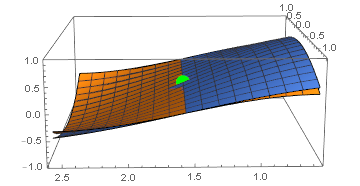
\includegraphics[scale=0.5]{2.ariketa Taylor-1.png}
    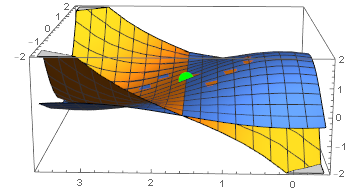
\includegraphics[scale=0.5]{2.ariketa Taylor-2.png}
    \label{fig:my_label}
\end{figure*}

\chapter{Aldagai anitzeko funtzioen analisi lokala}
\section{Aldagai anitzeko funtzioen mutur baldintzatuak}
\underline{19.ariketa} Zer luze dira azalera txikiena duen V bolumeneko paralelepipedoaren ertzak? Eta azalera handienekoarenak?

\begin{equation*}
    V = xyz
\end{equation*}
\begin{equation*}
    A(X,Y,Z) = 2xy + 2xz + 2zy = 2(xy+xz+xy)
\end{equation*}
\centering Funtzio laguntzailea(A eta $\lambda$ (V anulatuta)):
\begin{equation*}
    F(x,y,z) = (2xy + 2xz + 2zy) + \lambda(xyz-V)
\end{equation*}
\centering Hasteko puntu kritikoak bilatuko ditugu. Deribatu Partzialetatik hasiko gara:
\begin{equation*}
\left.
  \begin{tabular}{ c }
    $D_{1f}(x,y,z)=2(y+z) + \lambda(yz)$ \\
    $D_{2f}(x,y,z)=2(x+z) + \lambda(xz)$ \\
    $D_{3f}(x,y,z)=2(x+y) + \lambda(yx)$ \\
    $V = xyz$ 
    \end{tabular}
  \right\}
  \rightarrow
  \left.
  \begin{tabular}{ c }
    $2(y+z) + \lambda(yz) = 0$ \\
    $2(x+z) + \lambda(xz) = 0$ \\
    $2(x+y) + \lambda(yx) = 0$ \\
    $V = xyz$ 
  \end{tabular}
  \right\}
  \rightarrow
    \left.
  \begin{tabular}{ c }
    $\lambda = \frac{-2(y+z)}{yz}$ \\
    $\lambda = \frac{-2(x+z)}{xz}$ \\
    $\lambda = \frac{-2(x+y)}{yx}$ \\
  \end{tabular}
  \right\}
  \rightarrow
\end{equation*}
\centering Ekuazio sistema askatu:
\begin{equation*}
\rightarrow
  \left\{
  \begin{tabular}{ c }
     $\frac{-2(y+z)}{yz} = \frac{-2(x+z)}{xz} \rightarrow (y+z)xz=(x+z)yz \rightarrow z(yx+zx-yx-zy)=0$\\
     $\frac{-2(y+z)}{yz} = \frac{-2(x+y)}{xy} \rightarrow (y+z)xy=(x+y)yz \rightarrow xy^2 + xyz = xyz -y^2z$
  \end{tabular}
  \right.
  \rightarrow
\end{equation*}
\begin{equation*}
\rightarrow
  \left\{
  \begin{tabular}{ c }
    $z(zx-zy)=0 \rightarrow z^2(x-y)=0 \rightarrow \cancel{z=0} \text{ edo } x=y$ \\
    $xy^2 + xyz -xyz +y^2z=0 \rightarrow y^2(x+z)=0 \rightarrow \cancel{y=0} \text{ edo } x=-z$ \\
  \end{tabular}
  \right.
  \rightarrow
\end{equation*}
\begin{equation*}
 \rightarrow
 \left.
 \begin{tabular}{ c }
    $x=y=-z$ \\
    $V=xyz$ \\
  \end{tabular}
  \right\}
  \rightarrow
   \boxed{P(\sqrt[3]{V}, \sqrt[3]{V}, \sqrt[3]{V})}
\end{equation*}
\centering Puntuaren Izaera aztertuko dugu 
\newpage
\begin{equation*}
    \boxed{g(x,y) = F\Bigg(x,y,\frac{V}{xy}\Bigg)} = 2xy + 2x\Bigg(\frac{V}{xy}\Bigg) + 2y\Bigg(\frac{V}{xy}\Bigg)= 2xy + \frac{2V}{y} + \frac{2V}{x}
\end{equation*}
Segida Hessetarra lortu dugu:
\begin{itemize}
    \item $H_1$ lortu
        \begin{equation*}
        D_{1}g(x,y) = \frac{-2V}{x^2} + 2y
        \rightarrow
        D_{11}g(x,y) = \frac{4V}{x^3}
        \rightarrow
        \lambda_{1} = D_{11}g(\sqrt[3]{V}, \sqrt[3]{V}) = 4
        \end{equation*}
\item $H_2$ lortu
    \begin{equation*}
        D_{1}g(x,y) = \frac{-2V}{x^2} + 2y
        \rightarrow
        \left\{
        \begin{tabular}{c}
        $D_{11}g(x,y) = \frac{4V}{x^3}$ \\
        $D_{21}g(x,y) = 2$
        \end{tabular}
        \right.
    \end{equation*}
    \begin{equation*}
        D_{2}g(x,y) = \frac{-2V}{y^2} + 2x
        \rightarrow
        \left\{
        \begin{tabular}{c}
        $D_{12}g(x,y) = 2$ \\
        $D_{21}g(x,y) = \frac{4V}{x^3}$
        \end{tabular}
        \right.
    \end{equation*}
    \begin{equation*}
        H_2 = 
    \begin{vmatrix}
        D_{11g} & D_{12g}\\
        D_{21g} & D_{22g}
    \end{vmatrix}
    =
    \begin{vmatrix}
        \frac{4V}{x^3} & 2\\
        2 & \frac{4V}{x^3}
    \end{vmatrix}
    \end{equation*}
    \begin{equation*}
        \lambda_{2}(\sqrt[3]{V},\sqrt[3]{V}) = 
    \begin{vmatrix}
        4 & 2\\
        2 & 4
    \end{vmatrix}
    = 12
    \end{equation*}
\item Segida hesetarra
    \begin{equation*}
    \{1, \lambda_{1}, \lambda_{2}\} = \{1, 4, 12\}
    \rightarrow
    \boxed{\text{Minimoa }\Big(\sqrt[3]{V}, \sqrt[3]{V}, \sqrt[3]{V}, 6\cdot(\sqrt[3]{V})^2\Big)}
    \end{equation*}
\end{itemize}
\centering Minimo erlatibo baldintzatua.





\chapter{Integral mugagabea}
\underline{7.27.ariketa} Kalkulatu ondoko integral hau:
\begin{equation*}
    \int \frac{\sqrt{x}-\sqrt[6]{x}}{\sqrt[3]{x}+1}\ dx;
\end{equation*}

Integrala berehalakoa ez denez integrazio metodo bat erabili behar dugu, kasu honetan aldagai-aldaketa erabiliko dugu. 

\begin{equation*}
\biggr\rvert\hspace{0.1cm} x=t^6\hspace{0.5cm} dx=6t^5dt\hspace{0.1cm}\biggr\rvert
\end{equation*}

Balio berriak integralean ordezkatuko ditugu. 

\begin{equation*}
    \begin{split}
        \int \frac{\sqrt{x}-\sqrt[6]{x}}{\sqrt[3]{x}+1}\ dx = \int \frac{t^3-t}{t^2+1}6t^5dt = 6 \cdot \int \frac{t^8-t^6}{t^2+1}dt = \\ 6 \cdot \int \frac{(t^2+1)(t^6-2t^9+2t^2-2)+2}{(t^2+1)}dt = 6 \cdot \int t^6-2t^4+2t^2-2+\frac{2}{t^2+1}dt = 
    \end{split}
\end{equation*}

Integrala sinplifikatu ondoren berehalakoa bihurtzen da.

\begin{equation*}
     \begin{split}
        6 \cdot                  \left[\frac{t^7}{7}-\frac{2t^5}{-5}+\frac{2t^3}{3}-2t+2\cdot\int \frac{1}{t^2+1}dt\right] = \\ \frac{6}{7} \cdot t^7 - \frac{12}{5}t^5+4t^3-12t+12\arctan{t} + k =
    \end{split}
\end{equation*}
Bukatzeko ordezkatutako balioak desegin behar dira, lehengoko balioak sartuz. Hau da, $t$ jartzen duen lekuan $\sqrt[6]{x}$-rekin ordezkatu.

\begin{equation*}
    \frac{6}{7}\sqrt[6]{x^7}-\frac{12}{5}\sqrt[6]{x^5}+4+\sqrt{x}-12\cdot\sqrt[6]{x}+12\arctan{(\sqrt[6]{x})}+k
\end{equation*}


\chapter{Integral mugatua}
\section{Integral mugatuen aplikazioak}
\underline{13.7.ariketa} Kalkulatu ondoko funtzioak biratzean osatzen duen gorputzaren bolumena

\begin{equation*}
    x^2+(y-b)^2=a^2,\ \text{torua}\ b>a \ \text{izanik;}
    \end{equation*}
    \newline
    Ikusten dugunez, gorputz honek eragiten duen bolumena (kalkulatu behar dugun bolumena) hau izango litzateke, hau da, gorputza biratzean, gorputzak hutsune bat utziko du gorputza eta ardatzaren artean eta hori izango da kulatuko dugun zatia. 

    
   \begin{figure*}[h]
    
 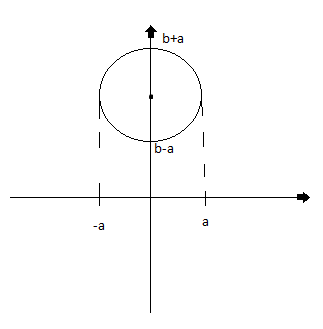
\includegraphics[scale=1]{4.png}
 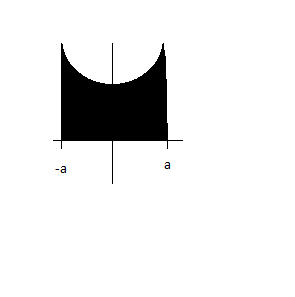
\includegraphics[scale=1.2]{4b.png}
    \end{figure*}
    \newpage
    
    
Horretarako formula hau erabiliko dugu bolumena kalkulatzeko:\\

$$V=\int_{-a}^{a} f^2(x)-g^2(x) dx$$\\
Formula honen bidez zilindroak osatzen duen gorputzaren bolumena kalkulatuko dugu, horretarako zilindroaren  zati positiboa eta negatiboaren kenketa egingo dugu ezkerreko marrazkian dugun gorputzaren bolumena kalkulatzeko:
$$V= \pi \int_{-a}^{a} (b+\sqrt{a^2-x^2})^2-(b-\sqrt{a^2-x^2})^2 dx$$

Garatu eta sinplifikatu:
$$V= \pi \int_{-a}^{a} (\cancel{b^2}+2b\sqrt{a^2-x^2}+\cancel{(a^2-x^2)})-(\cancel{b^2}-2b\sqrt{a^2-x^2}+\cancel{(a^2-x^2)}) dx=$$
$$V= \pi \int_{-a}^{a} 4b\sqrt{a^2-x^2} dx=  $$$$V= 4b\pi \int_{-a}^{a} \sqrt{a^2-x^2} dx$$\\
 
 Integral hau garatzeko IV motako integralen ebazpidea jarraitzen dugu.\\
 $$\text{1.}\sqrt{a^2-x^2} \text{agertzen bada, aldagai-aldaketa hau egingo dugu: x= a sin t}$$\\
 \centering$V= 4b\pi \int_{-a}^{a}\underline{\sqrt{a^2-x^2}}   dx =\text{I1} $\\
 
 $$  \hspace{1.5cm}                   \updownarrow$$
  

\begin{center}
\begin{tabular}{ c c  }
  &  $x=a \rightarrow a = a sin (t) \rightarrow sin(t)=1 \rightarrow \boxed{t=\frac{\pi}{2} }$  \\ 
 $x= a sin (t)$ &  \\  
  &  $x=-a \rightarrow -a = a sin (t) \rightarrow sin(t)=-1 \rightarrow \boxed{t=-\frac{\pi}{2}} $     
\end{tabular}
\end{center}

$dx = acos(t) dt$                         


 \newpage
 Aldagai aldaketa aplikatzen dugu balioak ordezkatuz eta ekuazio trigonometrikoak aplikatuz:
 \\
 \vspace{1cm}
 $ \text{I1 =}  \int\sqrt{a^2-x^2} dx = \int\sqrt{a^2-a^2sin(t)} \cdot acos(t) dt= \int\sqrt{a^2(1-sin^2(t))} \cdot acos(t)=   $
  
   \vspace{1cm}
 $\int\sqrt{a^2\cdot cos^2(t)}= acos(t) \cdot acos(t) dt   $
  \vspace{1cm}\\
Beraz, integrala honela geratuko litzakete(I1-ean ordezkatu):\\
 \vspace{1cm}
$V= 4b\pi \int_{-a}^{a}\underline{\sqrt{a^2-x^2}}   dx =\text{I1} \longrightarrow 4b\pi\int_{-\frac{\pi}{2}}^{\frac{\pi}{2}}acos(t) \cdot acos(t) dt \longrightarrow 4ba^2\pi\int_{-\frac{\pi}{2}}^{\frac{\pi}{2}} cos^2(t)dt =$\\
\vspace{1cm}


$4ba^2\pi\int_{-\frac{\pi}{2}}^{\frac{\pi}{2}}\frac{1+cos(2t)}{2} = 2ba^2\pi\int_{-\frac{\pi}{2}}^{\frac{\pi}{2}}1+cos(2t) dt =$\\
\vspace{1cm}
$2ba^2\pi\left[t+\frac{1}{2}\cdot sin(2t)   \right]_{-\frac{\pi}{2}}^\frac{\pi}{2} = 2ba^2\pi\left[(\frac{\pi}{2}+\frac{1}{2}\cdot sin(\pi) )-(-\frac{\pi}{2}+\frac{1}{2}\cdot sin(-\frac{\pi}{2})   \right] = \boxed{2ba^2\pi^2}$






 






    
    
    
    
    
    
    
    
